\documentclass[a4paper,10pt]{article}
\usepackage{mystyle}
\usepackage[top=3cm, bottom=3cm, left=3cm, right=3cm]{geometry}
\def\labelitemi{---}

\lstset{
    language=Python,
    frame=single,
    numbers=left,
    breaklines=true,
}

\begin{document}

\title{\texttt{PrefixCCFWC}: technical report}
\author{Victor Lecomte}
\maketitle

\begin{abstract}
In scheduling, it may be useful to specify cardinality constraints on some prefixes of an array of variables. For example, if the variables represent which product will be made each day, and you have to deliver 3 units of product $A$ after 7 days, you will want to impose that there be at least 3 occurences of $A$ among the first 7 variables.

This constraint allows you to apply many such constraints on several values without the overhead of creating a GCC for each of them, and with some additional pruning.
\end{abstract}

\tableofcontents

\section{Problem statement}
We are given an array of integer variables and a number of constraints of the form:
\begin{quote}
There should be at least $lb$ / at most $ub$ occurrences of value $v$ among the first $i$ variables.
\end{quote}
In scheduling this will mostly be lower bounds coming from quantities to be produced at a certain date, but there could also be upper bounds coming from storage limitations.

For example let's consider four variables with values either \texttt{A} or \texttt{B}, and the following constraints:
\begin{itemize}
    \item there should be at least one \texttt{B} in the first two variables ($lb=1$, $v=\texttt{B}$, $i=2$);
    \item there should be at most two \texttt{A}'s in all the variables ($ub=2$, $v=\texttt{A}$, $i=4$).
\end{itemize}
Then the following results would be valid:
\begin{itemize}
    \item \texttt{A B A B}
    \item \texttt{B B B B}
\end{itemize}
While the following results would be invalid:
\begin{itemize}
    \item \texttt{A A B B} (no \texttt{B} in the first two variables)
    \item \texttt{B A A A} (too many \texttt{A}'s)
\end{itemize}

\section{The algorithm}
The algorithm consists of two main parts:
\begin{enumerate}
    \item The deduction and filtering of the bounds, where we analyze the bounds given to filter out the redundant ones and add additional ones when possible.
    \item The propagation, which takes the bounds obtained in the first part and applies pruning identical to regular forward-checking GCC, but in an efficient unified manner.
\end{enumerate}

We will start by explaining the \emph{bound deduction} (\ref{subsec:deduction}) and \emph{bound filtering} (\ref{subsec:filtering}) steps, then we will introduce the concept of \emph{critical points} (\ref{subsec:critical}) and how it is the key in unifying the bound checking, and finally we will go on to the \emph{merging and pruning process} (\ref{subsec:merging-pruning}), the main propagation mechanism.

\subsection{Bound deduction}
\label{subsec:deduction}

The deduction step aims to obtain better bounds for the occurrences of a value than those given in the input, based on two factors:
\begin{itemize}
    \item the values of the bounds on the same value for other prefixes, which we will call \emph{inter-prefix} deduction;
    \item the values of the opposite bounds for the same prefix on other values, which we will call \emph{inter-value} deduction.
\end{itemize}

\subsubsection{Inter-prefix deduction}

The first factor is based on these four types of deduction:
\begin{itemize}
    \item if there are at least three \texttt{A}s in the first five variables, there are also at least three \texttt{A}s in the first six variables (I), and at least \emph{two} in the first four (because we are removing at most one) (II);
    \item if there are at most three \texttt{A}s in the first five variables, there are also at most three \texttt{A}s in the first four variables (III), and at most \emph{four} in the first six (because we are adding at most one) (IV).
\end{itemize}

In practice, those deductions can be made by maintaining an array of the best known bounds for each prefix and then traversing it once forwards for deductions (I) and (IV) and once backwards for deductions (II) and (III).

Here is a pseudocode, for a certain value:
\begin{lstlisting}
for i in 1 to (numberOfVariables):
    lower(i) = max(lower(i), lower(i-1))     # deduction (I)
    upper(i) = min(upper(i), upper(i-1) + 1) # deduction (IV)
for i in (numberOfVariables-1) to 0:
    lower(i) = max(lower(i), lower(i+1) - 1) # deduction (II)
    upper(i) = min(upper(i), upper(i+1))     # deduction (III)
\end{lstlisting}

\subsubsection{Inter-value deduction}

The second factor is based on these two types of deduction:
\begin{itemize}
    \item in the first five variables, if the \emph{minimal} number of occurrences for all the other values is three, then we can decrease the \emph{maximal} number of occurrences for this value to two (since there are at most five occurences in total);
    \item in the first five variables, if the \emph{maximal} number of occurrences for all the other values is three, then we can increase the \emph{minimal} number of occurrences for this value to two (since there are at least five occurrences in total).
\end{itemize}

In practice, those deductions can be made for each prefix and for each value by computing the sums of all the lower (resp. upper) bounds for all of the other values and setting the upper (resp. lower) bound of this value to the length of the prefix minus that sum (if this results in a stronger bound).

Here is a pseudocode, for a certain prefix:
\begin{lstlisting}
for v in values:
    lower(v) = max(lower(v), sizeOfPrefix - (sum(upper) - upper(v)))
    upper(v) = min(upper(v), sizeOfPrefix - (sum(lower) - lower(v)))
\end{lstlisting}

\subsection{Bound filtering}
\label{subsec:filtering}

Now that the we have deduced the best possible bounds for every prefix, we would like to filter them and only keep those that add information. We can see this step as applying the inter-prefix deduction in reverse: instead of creating new bounds by deducing them from the next or previous prefix, we will remove them if they can be deduced in that way.

In practice, we will traverse the prefixes from left to right, and:
\begin{enumerate}
    \item only add a bound if it gives more information than the previous bound;
    \item remove the previous bounds that can be deduced from the bound we're adding.
\end{enumerate}

Note that second point is similar in spirit to the ``monotone chain'' algorithm for convex hulls: we are trying to find a minimal set of bounds and to ensure it's minimal, when adding a new bound, we remove the previous bounds as long as they're being made useless by the new one. Only the criterion changes.

In the case of lower bounds, we use these deduction laws (see \ref{subsec:deduction}):
\begin{itemize}
    \item a bound only adds information if it is higher than the previous one (I);
    \item a previous bound has to be removed if it is lower or equal to the new bound \emph{minus their distance} (II).
\end{itemize}

For example, if we have a lower bound of one on the first three variables, we can add a lower bound of three on the first five variables, because it adds informations. However, we will then have to remove the previous constraint, because that lower bound of one can be directly deduced from the one we're adding.

In general, we can visually check if a lower bound is stronger than another by ``extending'' it, decreasing constantly on the left and staying constant on the right, as shown in figure~\ref{fig:lower-bounds}.

\begin{figure}[h!]
    \centering
    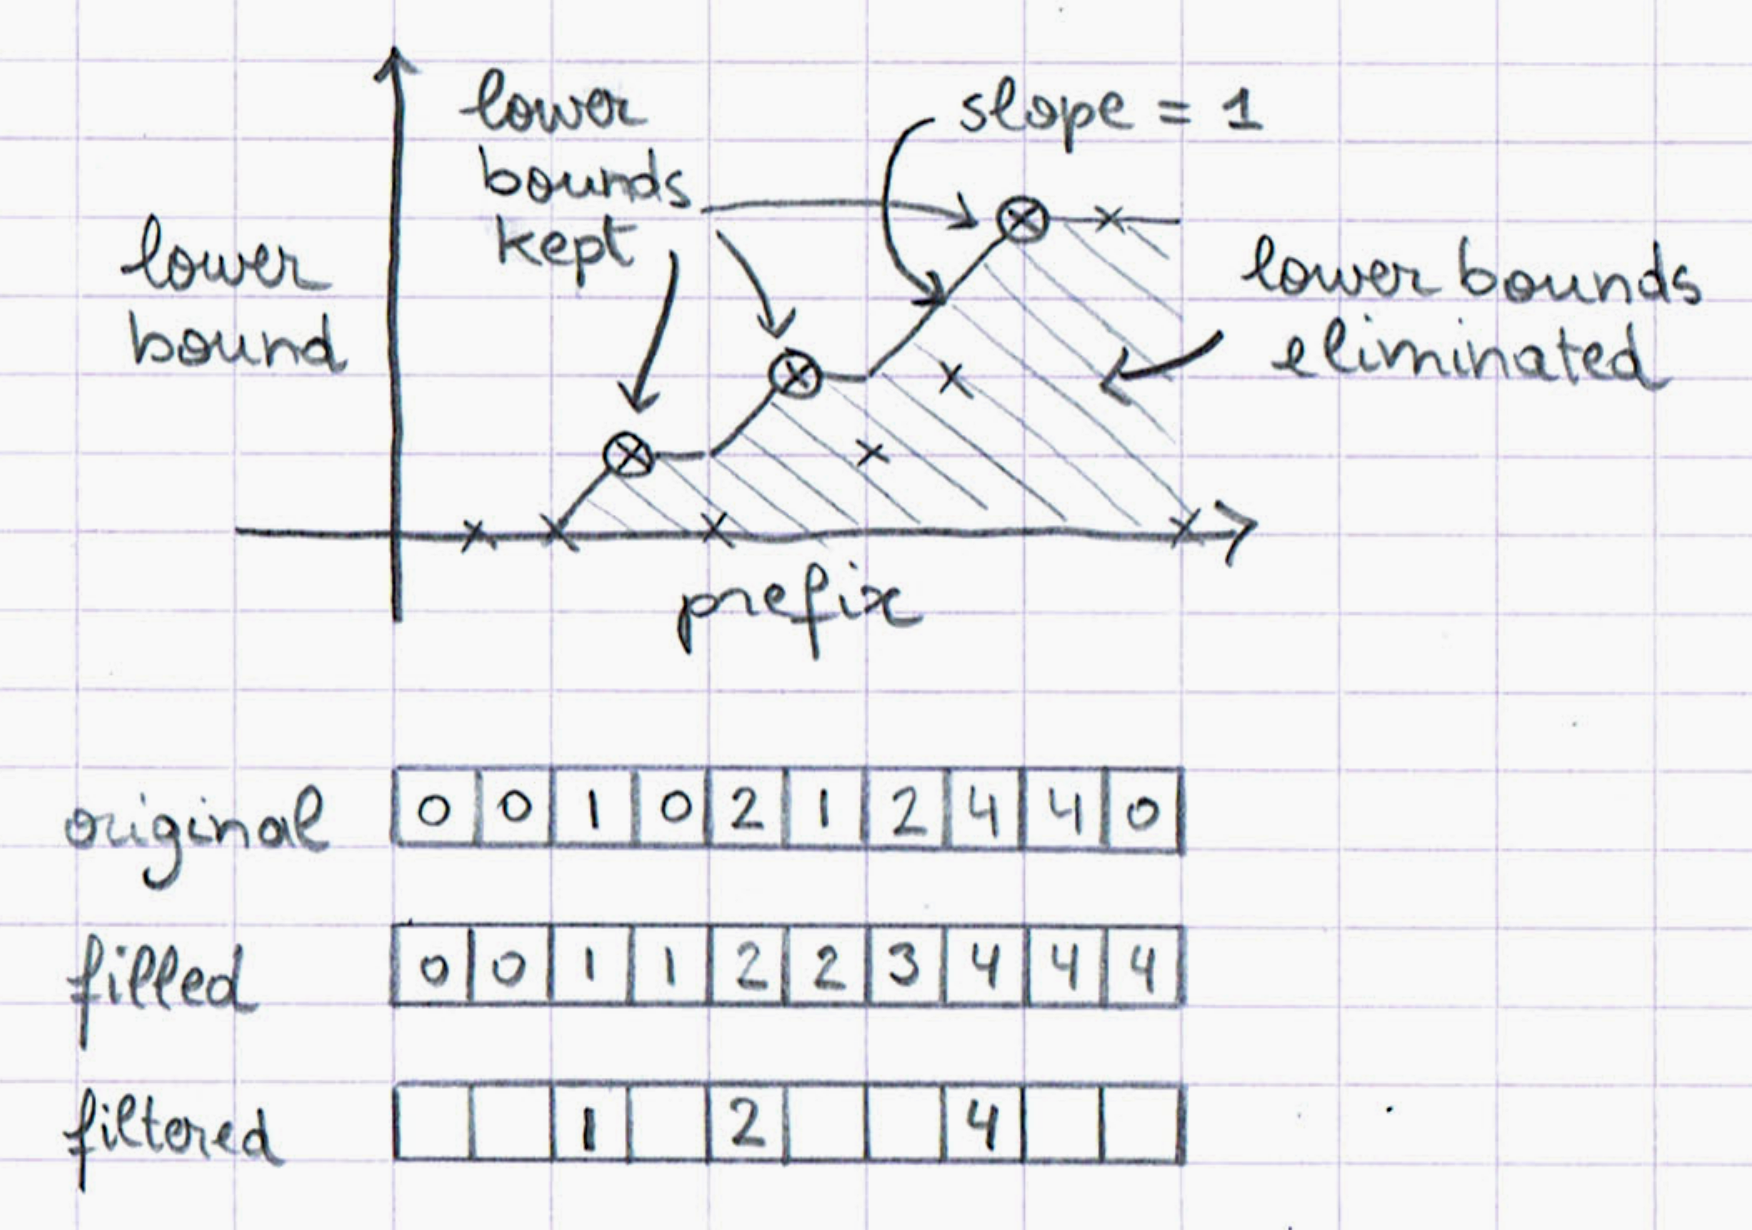
\includegraphics[width=0.7\textwidth]{img/lower-bounds}
    \caption{The selection of lower bounds \textbf{TODO: scan version with arrays}}
    \label{fig:lower-bounds}
\end{figure}

Here is a pseudocode of the filtering for lower bounds:
\begin{lstlisting}
for cur in lowerBounds:
    if cur.bound > last.bound:
        while last.bound <= cur.bound - (cur.index - last.index):
            removeLast()
        add(cur)
\end{lstlisting}

The situation is similar for upper bounds:
\begin{itemize}
    \item a bound only adds information if it is lower than the previous one \emph{plus their distance} (IV);
    \item a previous bound has to be removed if it is higher or equal to the new bound (III).
\end{itemize}

The visual extension works in a similar way, as shown in figure~\ref{fig:upper-bounds}.

\begin{figure}[h!]
    \centering
    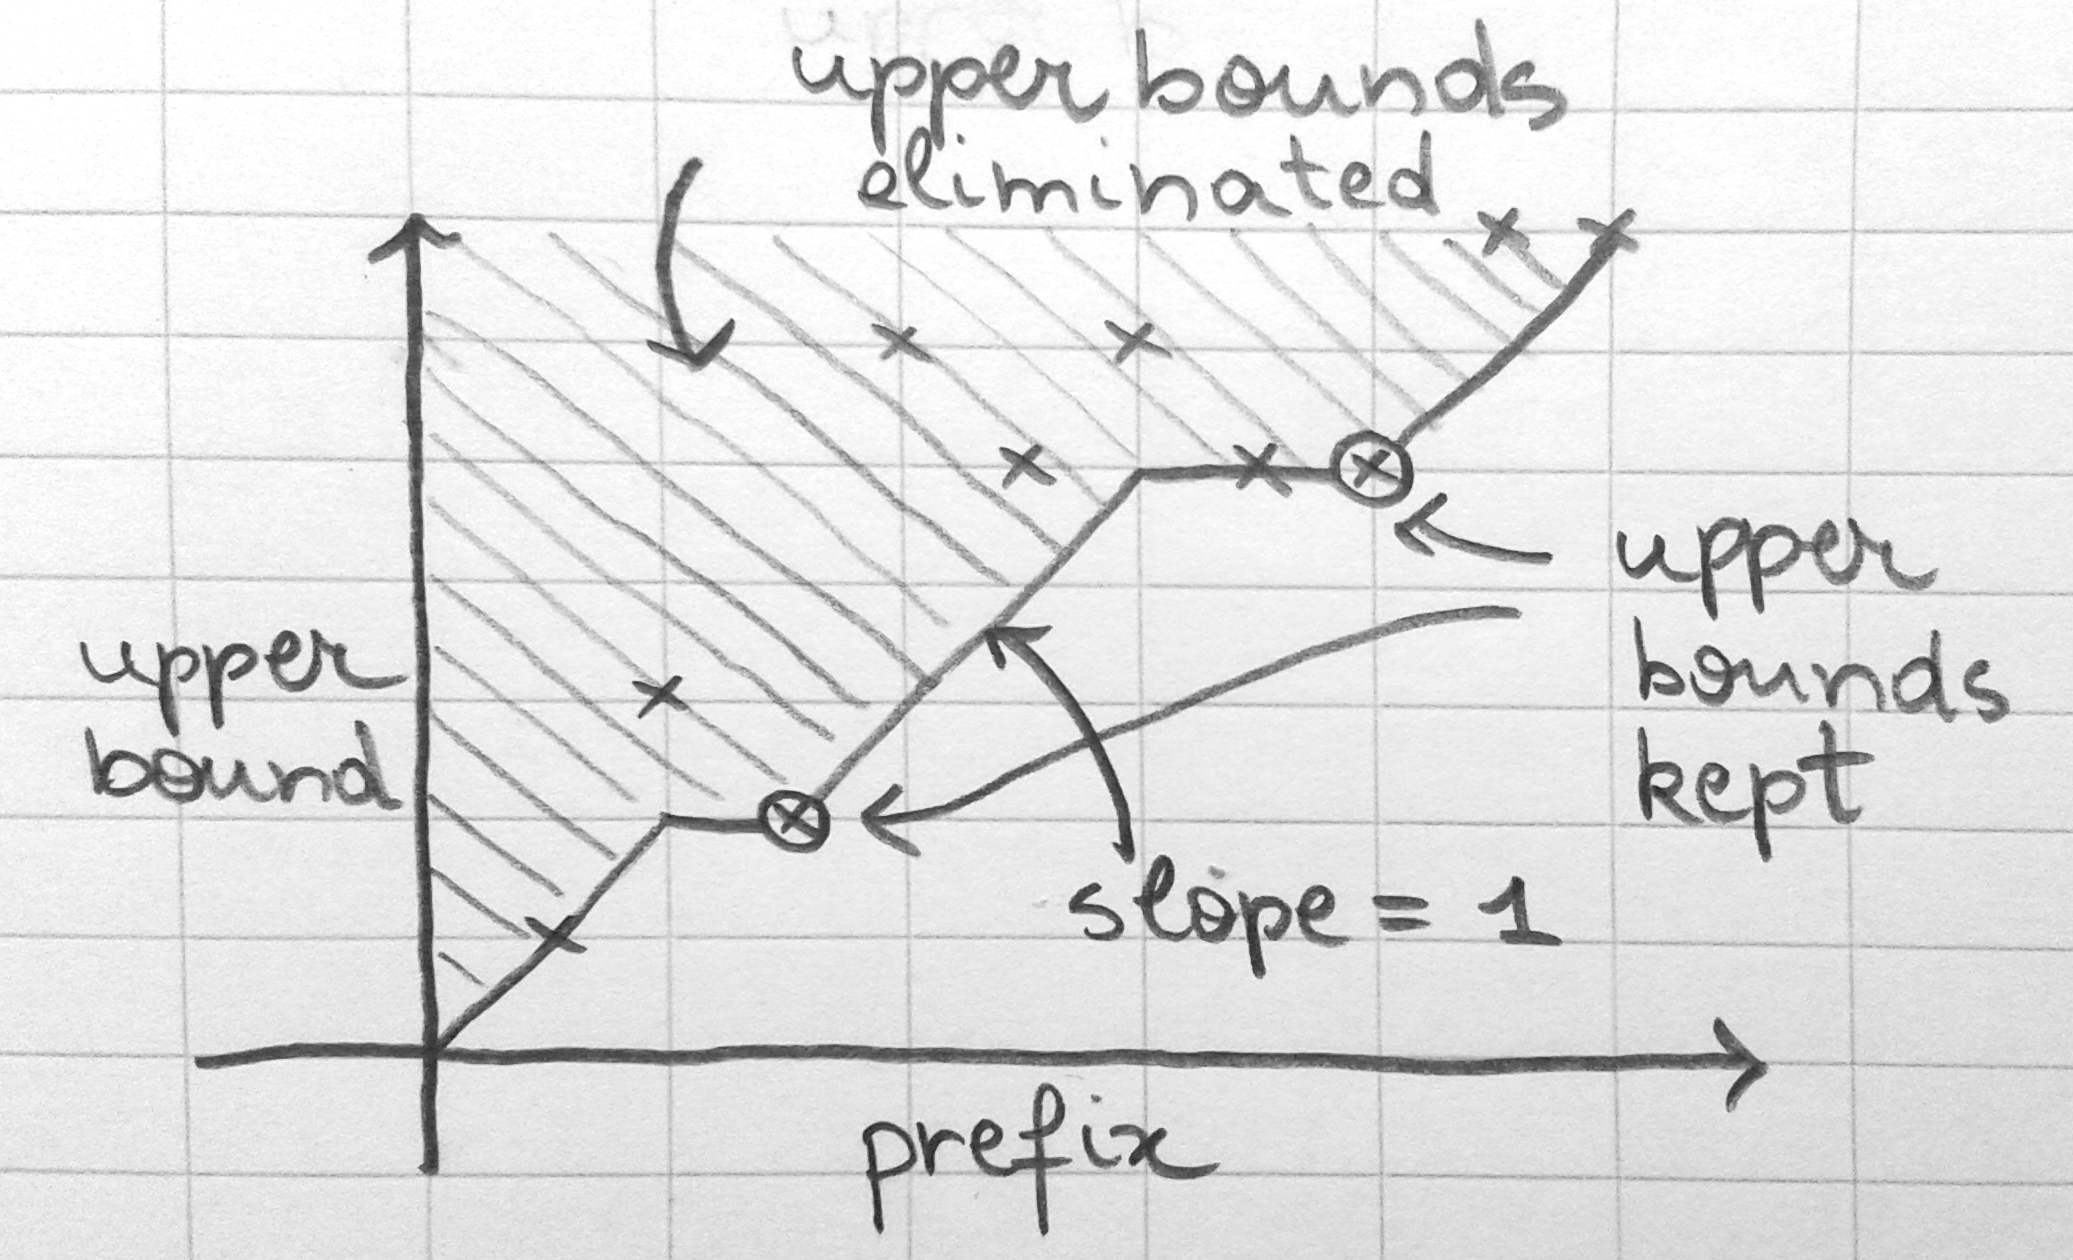
\includegraphics[width=0.6\textwidth]{img/upper-bounds}
    \caption{The selection of upper bounds \textbf{TODO: scan version with arrays}}
    \label{fig:upper-bounds}
\end{figure}

Here is a pseudocode of the filtering for upper bounds:
\begin{lstlisting}
for cur in upperBounds:
    if cur.bound < last.bound + (cur.index - last.index):
        while last.bound >= cur.bound
            removeLast()
        add(cur)
\end{lstlisting}

\subsection{The concept of critical points}
\label{subsec:critical}

Now that we have obtained an optimal set of bounds, we have to figure out how to quickly check when updating whether a bound has reached its objective: we want to know when the number of variables that have a value reaches the lower bound, so that we can assign them all; and when the number of variables that are bound to the value reaches the upper bound, so that we can remove the value from all the other variables.

The issue is that a variable may be included in many prefixes with a lower bound or an upper bound, and checking every single one of them could take time. We have to find a way to do it only once.

In order to do that, we divide the variables into the segments that are formed by the bounds. For example, if for some value we have an upper bound of 2 for the prefix $[0,3)$ and an upper bound of 5 for the prefix $[0,8)$, we will separate the variables into the segments $[0,3)$ and $[3,8)$.

Let us examine the differences between the bounds. If in the segment $[3,8)$ the number of variables bound to the value reaches $5-2=3$, that means there will be at least 3 occurrences of the value in that segment. As a consequence, if the upper bound of 2 in the prefix $[0,3)$ fails, there will be more than 2 occurrences of the value in $[0,3)$ and thus more than 5 occurrences in $[0,8)$, which makes the upper bound in the prefix $[0,8)$ also fail! Since the upper bound for $[0,3)$ can only fail when the other one also fails, it does not add any information anymore, and we can eliminate it.

We will name this difference $5-2=3$ the \emph{critical point} for that segment. It means that when the number of variables assigned to the value in the segment reaches that point, we can eliminate the bound on the left of the segment. When updating, our only job will then be to check whether we reached the critical point, and trigger actions if that is the case.

The critical point also makes sense for lower bounds: if this time we take a \emph{lower} bound of 2 for $[0,3)$ and a \emph{lower} bound of 5 for $[0,8)$, and the number of variables that have the value in the segment decreases to 3, that means there will be at most 3 occurrences of the value in that segment. As a consequence, if the lower bound of 2 in the prefix $[0,3)$ fails, there will be less than 2 occurrences of the value in $[0,3)$ and thus less than 5 occurrences in $[0,8)$, which makes the lower bound in the prefix $[0,8)$ also fail. Since the lower bound for $[0,3)$ can only fail when the other one also fails, it does not add any information anymore, and we can eliminate it.

So to each segment we attribute a critical point which is the difference of the bounds on its right and on its left. For the leftmost segment, we simply define the critical point to the bound on the right, which we can think of as the difference between that bound and a bound of 0 for $[0,0)$.

Since reaching the critical point eliminates the need for the bound on the left end of the segment, we can merge the segment with the one left of that bound. We then start tracking the progress towards the critical point on that larger segment.

\subsection{Merging and pruning}
\label{subsec:merging-pruning}

Now we have to use the idea of critical points and segments to determine when to prune, and in which prefix we have to assign or remove values from variables.

First we observe that, when we reach the critical point on the leftmost segment, we have to trigger pruning on it. For example, if we have an upper bound of 2 on the prefix $[0,3)$ and two variables in it have been assigned to the value, we have to remove the value from the third variable, otherwise it might create a third occurrence. Similarly, if it had been a lower bound and there were only two variables with the value, we would have had to assign them both.

Secondly we observe that we cannot prune any further than that segment: take that same example with another upper bound of 5 at $[0,8)$, if the segments have not yet been merged, it means that the critical point in $[3,8)$ has not yet been reached, and there are less than 5 variables assigned to the value in $[0,8)$, which is not enough to trigger pruning linked to that upper bound. Same goes for the lower bounds: there would still be more than 5 variables that have the value in $[0,8)$, and that is too much to trigger pruning.

Therefore, we realize that to obtain the same pruning as individual GCCs (\emph{after} the bound deduction), we only have to prune when the segment on the very left reaches its critical point, and when that happens we have to prune the variables of that segment and only there. Afterwards, we can merge that segment with the one on the right, because it becomes the next candidate for pruning. The rest of the time, when the critical point is reached, we just merge the segment with the one on the left.

In order to know which variables to prune, we keep an ordered list of the variables that have the value but are not bound to it, which we call the ``unbound list''. When pruning, they will be the only ones we have to consider.

So we have reduced the problem of determining what to prune to the problem of merging adjacent segments and determining in which segment a variable is. This problem can be solved easily using a union-find data structure.

Here is a pseudocode for the update value removals, with lower bound segments:
\begin{lstlisting}
unboundList.remove(variable)
segment = findLowerBoundSegment(variable)
segment.numHavingTheValue -= 1
if segment.numHavingTheValue == segment.criticalPoint:
    if segment.leftEnd == 0:
        for var in unboundList.upto(segment.rightEnd):
            var.assign(value)
        union(segment, segment.onRight)
    else:
        union(segment, segment.onLeft)
\end{lstlisting}

And for the update on variable bindings, with upper bound segments:
\begin{lstlisting}
unboundList.remove(variable)
segment = findUpperBoundSegment(variable)
segment.numBoundToTheValue += 1
if segment.numBoundToTheValue == segment.criticalPoint:
    if segment.leftEnd == 0:
        for var in unboundList.upTo(segment.rightEnd):
            var.removeValue(value)
        union(segment, segment.onRight)
    else:
        union(segment, segment.onLeft)
\end{lstlisting}

\section{Complexity}

To examine the algorithmic complexity of this algorithm, let us define $n$ as the number of variables and $u$ as the number of updates, that is, the sum of the number of value removals and the number of variable bindings over the whole search. Note that when we prune by assigning or removing a value from a variable, it counts in $u$ as well.

As a reminder, when the constraint receives an update, it has to:
\begin{itemize}
    \item find which segment the updated variable belongs to (a ``find'' operation);
    \item update the counter that checks if we are at the critical point yet (constant time);
    \item remove it from the list of unbound variables (constant time);
    \item if we reached the critical point and this is the leftmost segment, prune in the segment (constant time per variable pruned) then merge with the segment on the right (a ``union'' operation);
    \item if we reached the critical point and this is \emph{not} the leftmost segment, merge with the segment on the left (a ``union'' operation).
\end{itemize}

The fourth step above deserves more explanation: even though it can take $O(n)$ for one particular update to be processed, the variables that are pruned also count as updates, so it still counts as amortized constant time per update.

When we combine all of this, we discover that the amortized complexity is the number of updates times the cost of a union-find operation, so one would think that this would give $O(u\cdot\alpha(n))$. However, since this is constraint programming, we are working with a reversible union-find structure, and the same union-find operation could be repeated many times, so we cannot use the amortized constant time $O(\alpha(n))$ of union-find operations, but rather the $O(\log n)$ worst-case cost of ``find'' operations.

As a result, we obtain the complexity $O(u \log n)$ for the whole search, or an amortized complexity of $O(\log n)$ per update.

\section{Conclusion and use cases}

This algorithm gives a bit more pruning than individual GCCs and its running time depends logarithmically on the size of the problem instead of linearly on the number of bounds.

However, because of its complexity of implementation and the lightning speed of GCCFWCs, when used alone, we have only found it to be beneficial for larger test cases with several lower or upper bounds for each value. It could also be useful for average-sized cases where the number of nodes is made critical by other constraints and the additional pruning is valuable.

For more details, see the accompanying performance analysis.

\end{document}
